\subtop{Orthogonale Gitterlayouts}{-1.45}
\begin{itemize}[itemsep=-1pt]
	\item jeder Knoten hat höchstens Grad $4$
	\item Algorithmus von Biedl und Kant (vier Schritte):
		\begin{enumerate}
			\item Zerlegung des Graphen in Komponenten
			\item Bestimmung der Reihenfolge für die Knoten jeder Komponente
			\item inkrementelle Bestimmung des Layouts für jede Komponente: die Knoten werden in ihrer Reihenfolge in das Layout eingefügt
			\item Kombinierung der Layouts der einzelnen Komponenten
		\end{enumerate}
	\item der Graph wird zuerst in hinreichend zusammenhängende Teilgraphen zerlegt
\end{itemize}
\subsection{Zweifache Zusammenhangskomponenten}
\begin{itemize}[itemsep=-1pt]
	\item Zwei Kanten in einem ungerichteten Graphen heißen \textit{biconnected}, wenn sie auf einem einfachen Kreis liegen.
	\item eine zweifache Zusammenhangskomponente wird auch als \textit{Block} bezeichnet
	\item aus einem zweifach zusammenhängenden Graphen müssen mindestens zwei Knoten entfernt werden, damit der Graph nicht mehr zusammenhängend ist
	\item die zweifachen Zusammenhangskomponenten können in Linearzeit berechnet werden,\algobreak\algo{BICOMP}{\begin{algorithm}[H]
	\SetAlgoVlined
	\SetKwProg{Fn}{Function}{}{end}
	\SetKwFunction{dfs}{dfs}
	\KwIn{ungerichteter Graph $G=(V,E)$}
	\KwData{Zähler $i$ für DFS-Nummerierung der Knoten\\Stack $S$ für nicht klassifizierte Kanten\\Stack $C$ der Repräsentaten auf aktuellem DFS-Weg}
	\KwOut{DFS-Nummern (Knoten, Kanten), Blockrepräsentant $BICOMP$ zu jeder Kante}
	\BlankLine
	\Fn{\dfs{vertex $v$}}{
		$i\leftarrow i+1$\\
		$DFS[v]\leftarrow i$\\
		\While{$\exists$ unnumerierte Kante $e=\{v,w\}$}{
			$DFS[e]\leftarrow DFS[v]$;\\
			$\push(e,S)$;\\
			\eIf{$w$ unnummeriert}{
				$\push(e,C)$;\\
				$\DFS(w)$; \\
				$[$Backtracking$]$ \\
				\If{$e=top(C)$}{
					\Repeat{
						$e'\leftarrow \pop(S)$
					}{
						$e'=e$;
					}
					$\pop(C)$;
				}
			}{
				\While{$DFS[top(C)]>DFS[w]$}{
					$\pop(C)$;
				}
			}
		}
	}
	\Begin{
		$i\leftarrow 0$;\\
		\ForEach{$s\in V$}{
			\If{$s$ unnumeriert}{
				$\DFS(s)$;
			}
		}
	}
\end{algorithm}}
	\vspace*{-1.25\baselineskip}
	\ProofIdea
		\vspace*{-1\baselineskip}
		per Induktion über die Anzahl der Kantendurchläufe:
			\begin{itemize}[itemsep=-1pt]
				\item eine Kante heißt \textit{offen}, wenn noch kein Backtracking erfolgt ist
				\item eine Kante heißt \textit{fertig}, falls Backtracking erfolgt ist
				\item eine Komponente heißt offen / fertig, falls ihre erste Kante offen / fertig ist
				\item $G_t$ ist der durch die nummerierten Kanten induzierte Teilgraph nach $t$ Kantendurchläufen
				\item offene Zusammenhangskomponenten werden als $G_t^{(i)}$, seine ersten Kanten als $E_t^{(i)}$ mit $e_i^{(i)}, 1\leq i\leq k_t$ in der Reihenfolge, wie sie markiert wurden
				\item zu Zeigen sind die folgenden Invarianten:
					\begin{enumerate}[itemsep=-1pt]
						\item alle Kanten einer fertigen Zusammenhangskomponenten zeigen auf die erste Kante der Komponente
						\item auf dem Stack $C$ liegen (von unten nach oben) $e_t^{(1)},\dots,e_t^{(k_t)}$
						\item auf dem Stack $S$ bilden die Kanten aus $E_t^{(1)},\dots,E_t^{(k_t)}$ Intervalle (in dieser Reihenfolge)
					\end{enumerate}
			\end{itemize}
\end{itemize}
\topbreak
\vspace*{-3.75\baselineskip}
\begin{itemize}
	\item[]\ \\
		\begin{itemize}
				\item alle Aussagen sind am Anfang richtig, bleibt zu zeigen dass sie auch für $t>0$, nach $t-1$ Durchläufen gelten (zwei Fälle):
					\begin{enumerate}
						\item Vorwärtsdurchlauf:\\
							\begin{minipage}{0.3\textwidth}
							\usetikzlibrary{positioning,patterns,arrows}
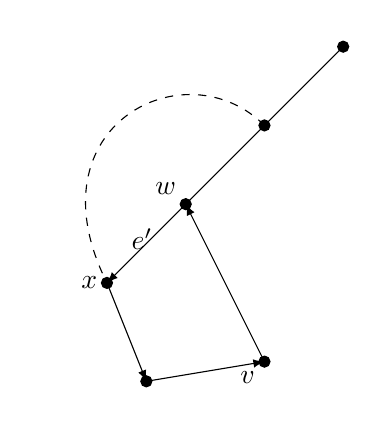
\begin{tikzpicture} [every node/.style={},node distance=0.2cm]

\coordinate[label={160:$w$}] (w) at (0,0);
\draw[fill](w) circle[radius=2pt];
\coordinate[label={180:$x$}] (x) at (-1,-1);
\draw[fill](x) circle[radius=2pt];
\coordinate[label={185:$v$}] (v) at (1,-2);
\draw[fill](v) circle[radius=2pt];

\coordinate[label={160:}] (v1) at (1,1);
\draw[fill](v1) circle[radius=2pt];
\coordinate[label={160:}] (v2) at (2,2);
\draw[fill](v2) circle[radius=2pt];
\coordinate[label={160:}] (v3) at (-.5,-2.25);
\draw[fill](v3) circle[radius=2pt];

\draw[-](v2)--(v1)--(w);
\draw[->,>=latex](w)to node [above left,xshift=0.2cm,yshift=-0.2cm] {$e'$}(x);
\draw[->,>=latex](x)to(v3);
\draw[->,>=latex](v3)to(v);
\draw[->,>=latex](v)--(w);

\draw[dashed] (1,1) .. controls (0,2) and (-2,1) .. (-1,-1);
\end{tikzpicture}
							\end{minipage}
							\begin{minipage}{0.55\textwidth}
								\begin{itemize}[itemsep=-1pt]
									\item[$\RHD$] $e$ ist Baumkante\\
									$\Rightarrow w$ ist Knoten vom Grad $1$ in $G_t\\
									\Rightarrow e$ ist einzige Kante einer neuen offenen Komponente\\
									$\Rightarrow$ alle Invarianten gelten
									\item[$\RHD$] $e$ ist Rückwärtskante zum Knoten $w\\
									\Rightarrow e$ bildet zusammen mit dem letzten (bei $w$ beginnenden) Teilstück des Weges der offenen Kanten einen einfachen Kreis\\
									$\Rightarrow$ alle Kanten auf diesem Kreis gehören zur gleichen Zusammenhangskomponente von $G_t$\\
									$\Rightarrow$ alle nach $e$ durchlaufenen Kanten werden aus $C$ entfernt\\
									$\Rightarrow$ alle Invarianten gelten
								\end{itemize}
							\end{minipage}
						\item Backtracking:
							\begin{itemize}[itemsep=-1pt]
								\item[$\RHD$] $e$ wird fertig\\
								$\Rightarrow$ durch 2. Invariante: $e$ erste Kante der offenen Komponente $\Leftrightarrow$ sie liegt oben auf $C$
								\item[$\RHD$] es gibt keine Quer- oder Vorwärtskanten in der ungerichteten Tiefensuche\\
								$\Rightarrow$ die Zusammenhangskomponente kann nicht mehr größer werden\\
								$\Rightarrow$ Zusammenhangskomponente ist fertig
								\item[$\RHD$] durch 3. Invariante werden durch die \textbf{repeat}-Schleife die richtigen Kanten von $S$ entfernt\\
								$\Rightarrow$ die Invarianten gelten
							\end{itemize}
						\item[$-$] Linearzeit: jede Kante wird höchstens einmal auf $C$ und $S$ gelegt
					\end{enumerate}
			\end{itemize}
\end{itemize}

\subsection{Knotenreihenfolge bestimmen (2. Schritt)}
\begin{minipage}{0.3\textwidth}
	\usetikzlibrary{positioning,patterns,arrows}
\begin{tikzpicture} [every node/.style={},node distance=0.2cm]

\newcommand{\nc}[4]{
	\coordinate[label={#4:$#1$}](#1) at (#2,#3) ;
	\draw[fill](#1)circle[radius=2pt];
}

\foreach[count=\c] \x/\y/\a in {0/0/270,-4/0/180,0/2/0,-6/2/180,-2/2/0,-4/4/160,-2/5/90}{
	\nc{\c}{0.75*\x}{0.75*\y}{\a}
}
\draw  (1) edge (2);
\draw  (1) edge (3);
\draw  (2) edge (4);
\draw  (2) edge (5);
\draw  (3) edge (7);
\draw  (4) edge (6);
\draw  (5) edge (6);
\draw  (6) edge (7);
\node (s) [right=of 1,xshift=-0.2cm]{$s$};
\node (t) [right=of 7,xshift=-0.15cm]{$t$};

\end{tikzpicture}
\end{minipage}
\begin{minipage}{0.6\textwidth}
	\begin{itemize}[itemsep=-1pt]
		\item der Algorithmus nutzt die \textit{$st$-Ordnung} als Reihenfolge der einzufügenden Knoten
		\item eine \textit{$st$-Ordnung} ist wie folgt definiert:
			\[\exists~ 1\leq i<j <k\leq n\text{ mit }\{v_i,v_j\},\{v_j,v_k\}\in E\]
		\item $G=(V,E)$, zweifach zusammenhängender Graph $\Leftrightarrow \exists$ zu jeweils zwei Knoten $s\neq t\in V$ eine $st$-Ordnung
	\end{itemize}
\end{minipage}\\
\begin{itemize}[itemsep=-1pt]
	\item durch eine \textit{Orientierung} erhält jede Kante in einem Graphen eine Richtung
	\item eine $st$-Orientierung ist azyklisch mit $s,t$ als einzige Quelle/Senke
	\item eine $st$-Ordnung kann mithilfe von \textit{topologischer Sortierung} aus einer $st-$Orientierung in Linearzeit berechnet werden
\end{itemize}
\topbreak
\vspace*{-2\baselineskip}
\subsubsection{Ohrendekomposition}
\begin{minipage}{0.3\textwidth}
	\usetikzlibrary{positioning,arrows,calc,patterns,snakes}

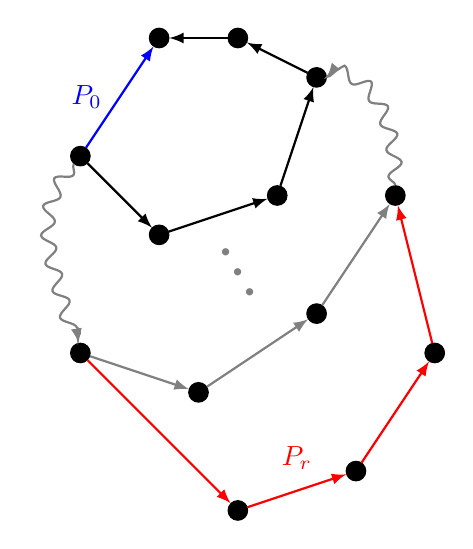
\begin{tikzpicture}[every node/.style={draw,circle,fill},scale=0.5]

\node[scale=0.75](1) at (0,4) {};
\node[scale=0.75](2) at (-2,1) {};
\node[scale=0.75](3) at (0,-1) {};
\node[scale=0.75](4) at (3,0) {};
\node[scale=0.75](5) at (4,3) {};
\node[scale=0.75](6) at (2,4) {};
\node[scale=0.75](7) at (-2,-4) {};
\node[scale=0.75](8) at (1,-5) {};
\node[scale=0.75](9) at (4,-3) {};
\node[scale=0.75](10) at (6,0) {};
\node[scale=0.75](11) at (2,-8) {};
\node[scale=0.75](12) at (5,-7) {};
\node[scale=0.75](13) at (7,-4) {};

\foreach[count=\c] \x/\y in {2/1,2/3,3/4,4/5,5/6,6/1}{
	\ifnum\c=1{
		\draw[->,>=latex,thick,color=blue](\x)to node[draw=none,fill=none,left] {$P_0$}(\y);
	}
	\else{	
		\draw[->,>=latex,thick](\x)--(\y);
	}\fi
}
\draw[->,>=latex,thick,decorate, decoration={snake},color=black!50](2)to[out=230,in=100](7);
\foreach[count=\c] \x/\y in {7/8,8/9,9/10}{
	\draw[->,>=latex,thick,color=black!50](\x)--(\y);
}
\draw[->,>=latex,thick,decorate, decoration={snake},color=black!50](10)to[out=90,in=0](5);

\foreach[count=\c] \x/\y in {7/11,11/12,12/13,13/10}{
	\ifnum\c=2{
		\draw[->,>=latex,thick,color=red](\x)to node[fill=none,draw=none,above] {$P_r$}(\y);
	}
	\else{
		\draw[->,>=latex,thick,color=red](\x)--(\y);
	}\fi
}

\node[draw=none,fill=none,color=black!50]at(2,-2){\Huge$\cdot$};
\node[draw=none,fill=none,color=black!50]at(2.3,-2.5){\Huge$\cdot$};
\node[draw=none,fill=none,color=black!50]at(1.7,-1.5){\Huge$\cdot$};

\end{tikzpicture}
\end{minipage}
\begin{minipage}{0.65\textwidth}
	\begin{itemize}[itemsep=-1pt]
		\item die Folge $D=(P_0,\dots,P_r)$ von (offenen) Pfaden heißt \textit{(offene) Ohrendekomposition}, falls
			\begin{itemize}[itemsep=-1pt]
				\item für $G_i=(V_i,E_i)$ gilt $V_i=\bigcup\limits_{j=0}^{i}V(P_j)$\\
				und $E_i=\bigcup\limits_{j=0}^{i}E(P_j)$, $0\leq 1\leq r$
				\item $E(P_0),\dots,E(P_r)$ ist eine Partition von $E$
				\item für alle $P_i=(v_0,e_1,v_1,\dots,e_k,v_k), 1\leq i\leq r$ gilt
					\begin{itemize}
						\item[$\RHD$] $\{v_0,v_k\}\subseteq V_{i-1}$
						\item[$\RHD$] $\{v_1,\dots,v_{k-1}\}\cap V_{i-1}=\emptyset$
					\end{itemize}
			\end{itemize}
		\item eine Ohrendekomposition beginnt mit der Kante $\{s,t\}\in E$, wenn $P_0=(s,\{s,t\},t)$
	\end{itemize}
\end{minipage}
\vspace*{-\baselineskip}
\begin{itemize}[itemsep=-1pt]
	\item für jeden zweifach zusammenhängenden Graphen gibt es für jede Kante $e=\{s,t\}$ eine Ohrendekomposition, die mit $e$ beginnt
	\item es kann in Linearzeit eine $st$-Orientierung aus einer offenen Ohrendekomposition konstruiert werden, die mit $\{s,t\}$ beginnt
		\vspace*{-1.5\baselineskip}
		\Proof
		\vspace*{-\baselineskip}
		Durch Konstruktion:
			\begin{itemize}[itemsep=-1pt]
				\item aus $P_0,\dots,P_r$, beginnend mit $\{s,t\}$, wird eine $st$-Orientierung konstruiert, indem
					\begin{itemize}[itemsep=-1pt]
						\item[$\RHD$] $P_0$ von $s$ nach $t$ orientiert wird
						\item[$\RHD$] $P_i=(u,\dots,w),1\leq i,\leq r$ von $u$ nach $w$ orientiert wird, falls $u$ in der von $P_0,\dots,P_{i-1}$ induzierten partiellen Ordnung vor $w$ liegt, sonst umgekehrt
					\end{itemize}
			\end{itemize}
	\item] Weg von der Ohrendekomposition zu einer $st$-Ordnung: \begin{center}\usetikzlibrary{positioning,arrows,calc,patterns,snakes}

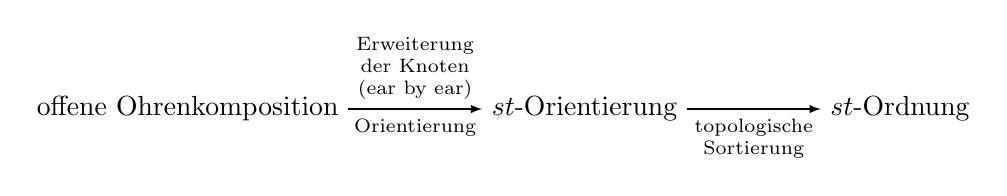
\begin{tikzpicture}[every node/.style={}]
\node[anchor=east] (v1) at (-3,0) {offene Ohrenkomposition};
\node (v2) at (0,0) {$st$-Orientierung};
\node[anchor=west] (v3) at (3,0) {$st$-Ordnung};

\draw[->,>=latex] (v1) to node[above]{\begin{minipage}{1.75cm}
\centering \scriptsize Erweiterung\\der Knoten\\(ear by ear)
\end{minipage}} node[below]{\scriptsize Orientierung} (v2);

\draw[->,>=latex] (v2) to node[below]{
\begin{minipage}{1.75cm}
\centering \scriptsize topologische Sortierung
\end{minipage}} (v3);


\end{tikzpicture}\end{center}
	\item Bestimmung einer Ohrendekomposition durch einen \textit{Tiefensuchbaum}:
		\begin{itemize}[itemsep=-1pt]
			\item Baumkanten $\{v,w\}$ werden als $v\rightarrow w$ bezeichnet
			\item Rückwärtskanten $\{v,w\}$ werden als $v\hookrightarrow w$ bezeichnet
			\item ein $uv$-Pfad mit höchstens Baumkanten wird als $u\overset{*}{\rightarrow}v$ bezeichnet
			\item Konstruktion der Ohrendekomposition:
				\begin{enumerate}[itemsep=-1pt]
					\item $P_0$ ist das Anfangsohr
					\item $\exists v\hookrightarrow w \notin E_i$ nach Konstruktion von $P_0,\dots,P_i,i\geq 0$\\
						$\Rightarrow P_{i+1}$ ist wie folgt definiert ($v,w,x \in V$):\\
						\begin{minipage}{0.4\textwidth}
							\usetikzlibrary{positioning,arrows,calc,patterns,snakes}

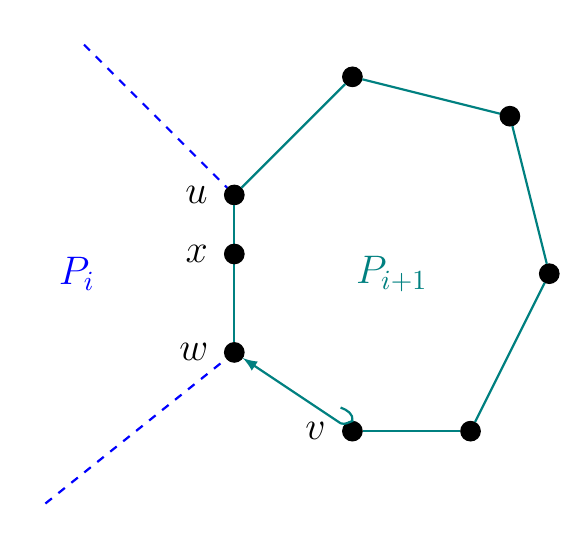
\begin{tikzpicture}[every node/.style={draw,circle,fill},node distance=0cm]

\node[draw=none,fill=none,scale=0.75] (v1) at (-4*0.5,4*0.5) {};
\node[scale=0.75] (v2) at (0,0) {};
\node[scale=0.75] (v4) at (0,-4*0.5) {};
\node[draw=none,fill=none,scale=0.75] (v3) at (-5*0.5,-8*0.5) {};
\node[scale=0.75] (v5) at (3*0.5,3*0.5) {};
\node[scale=0.75] (v6) at (7*0.5,2*0.5) {};
\node[scale=0.75] (v7) at (8*0.5,-2*0.5) {};
\node[scale=0.75] (v8) at (6*0.5,-6*0.5) {};
\node[scale=0.75] (v9) at (3*0.5,-6*0.5) {};

\draw[dashed,thick,color=blue] (v1) edge (v2);
\draw[dashed,thick,color=blue] (v3) edge (v4);

\foreach \x/\y in {2/5,5/6,6/7,7/8,8/9,4/2}
	\draw[thick,color=blue!50!green](v\x)to(v\y);
\coordinate (a) at (2.7*0.5,-5.8*0.5);
\coordinate (b) at (2.7*0.5,-5.4*0.5);
\draw[->,>=latex,thick,color=blue!50!green](b)to[out=340,in=80](v9.north)to[out=200,in=340](a)to(v4);

\node[draw=none,fill=none,color=blue] at (-4*0.5,-2*0.5) {\Large$P_i$};
\node[draw=none,fill=none,color=blue!50!green] at (4*0.5,-2*0.5) {\Large$P_{i+1}$};
\node[scale=0.75] (v10) at (0,-1.5*0.5) {};
\node[draw=none,fill=none,left=of v9] {\Large$v$};
\node[draw=none,fill=none,left=of v4] {\Large$w$};
\node[draw=none,fill=none,left=of v10] {\Large$x$};
\node[draw=none,fill=none,left=of v2] {\Large$u$};

\end{tikzpicture}
						\end{minipage}
						\begin{minipage}{0.55\textwidth}
							\begin{itemize}
								\item[$\RHD$] $w,x\in V_i$ 
								\item[$\RHD$] $v\hookrightarrow w\notin E$
								\item[$\RHD$] $w\rightarrow x$
								\item[$\RHD$] $x\overset{*}{\rightarrow}v$
								\item[$\RHD$] ist $u$ der letzte Knoten auf $x\overset{*}{\rightarrow}v$ mit $u\in V_i$ ($u=v$ ist möglich)\\
								$\Rightarrow P_{i+1}=u\overset{*}{\rightarrow}v\hookrightarrow w$
								\item[$\RHD$] aus $w\rightarrow x\overset{*}{\rightarrow}u$ folgt, dass $P_{i+1}$ offen ist ($P_{i+1}$ ist \textit{das Ohr zu} $v\hookrightarrow w$, \textit{trivial}, falls $u=v$)
							\end{itemize}
						\end{minipage}
				\end{enumerate}
		\end{itemize}
\end{itemize}
\topbreak
\vspace*{-2\baselineskip}
\begin{itemize}[itemsep=-1pt]
	\item eine offene Ohrendekomposition $D(T)=(P_0,\dots,P_r)$ überdeckt $G=(V,E)$ vollständig\\
	$\Rightarrow V=V_r,E=E_r$:
		\vspace*{-1.5\baselineskip}
		\ProofIdea
		\vspace*{-\baselineskip}
			Mit der zweifach Verbundenheit des Graphen kann man durch Konstruktion mithilfe eines Knotens $u\notin V_r$ einen Widerspruch herbei führen.
	\item die Ohren werden aufgrund der Orientierung der zugehörigen Baumkante orientiert, in der Reihenfolge von $D(T)$
	\item die Dekomposition definiert für jedes $i=0,\dots, r$ eine partielle Ordnung (reflexiv, transitiv, antisymmetrisch, nicht für alle Paare definiert - sonst total)
	\[\prec_i : \{v,w\}\in E_i \text{ von }v\text{ nach }w\text{ orientiert }\Rightarrow v\prec_i w\]
	\item die Orientierung von $D(T)$ liefert eine $st$-Orientierung von $G$
	\item die erhaltene Ordnung von $V_i$ ist eine lineare Erweiterung von $\prec_j$ für alle $0\leq j\leq i$ ($\prec_j\subseteq \prec_i$)\\
	$\Rightarrow$ die Ordnung ist eine $st$-Ordnung von $G$
	\item \algobreak\algo{$st$-Ordnung}{\begin{algorithm}[H]
	\SetAlgoVlined
	\SetKwProg{Fn}{Function}{}{end}
	\SetKwFunction{pe}{process\_ears}
	\SetKwFunction{dfs}{dfs}
	\KwIn{ungerichteter Grpah $G=(V,E)$, Kante $\{s,t\}\in E$}
	\KwData{ausgehende Baumkanten $CHILDEDGE$ für Knoten\\Vorgängerknoten $PARENT$ für Knoten\\Pfad $P$ (aktuelles Ohr)\\abhängige Nichtbaumkanten $D$ von Baumkanten}
	\KwOut{Liste $L$ der Knoten in Bicomp. von $\{s,t\}$ (in der $st$-Ordnung)}
	\BlankLine
	\Fn{\pe{Baumkante $w\rightarrow x$}}{
		\ForEach{$v\hookrightarrow w\in D[w\rightarrow x]$}{
			$u\leftarrow v$; %\\
			\While{$u\notin L$}{
				$u \leftarrow PARENT[u]$
				\tcp*[r]{Pfad zurückgehen, bis zu altem Ohr,\\das schon in $L$(orientiert) ist}
			}
			$P\leftarrow(u\overset{*}{\rightarrow}v \hookrightarrow w)$;\\
			\If{$w\rightarrow x$ von $w$ nach $x$ (oder $x$ nach $w$) orientiert ist}{
				orientiere $P$ von $w$ nach $x$ (oder $x$ nach $w$);\\
				füge inneren Knoten von $P$ unmittelbar vor (oder hinter) $u$ in $L$ ein;
			}
			\ForEach{Baumkante $w'\rightarrow x'$ von $P$}{
				\processears($w'\rightarrow x'$)
			}
		}
		$D[\{w,x\}]\leftarrow \emptyset$;
	}
	\Fn{\dfs{vertex $v$}}{
			$i\leftarrow i+1$\\
			$DFS[v]\leftarrow i$\\
			\While{$\exists$ unnumerierte Kante $e=\{v,w\}$}{
				$DFS[e]\leftarrow DFS[v]$;\\
				\eIf{$w$ unnummeriert}{
					$CHILDEDGE[v]\leftarrow e$;\\
					$PARENT[w]\leftarrow v$;\\
					$\DFS(w)$;
				}{
					$\{w,x\}\leftarrow CHILDEDGE[w]$;\\
					$D[\{w,x\}]\leftarrow D[\{w,x\}]\cup \{e\}$;\\
					\If{$x\in L$}{
						\processears($w\rightarrow x$);
					}
				}
			}
		}
	\Begin{
		Initialisieren von $L$ mit $s\rightarrow t$;\\
		$DFS[s]\leftarrow 1$;\\
		$i\leftarrow 1$;\\
		$DFS[\{s,t\}]\leftarrow 1$;\\
		$CHILDEDGE[s]\leftarrow \{s,t\}$;\\
		\DFS(t);
	}
\end{algorithm}}
\end{itemize}

\subsection{Layout einer Komponente (3. Schritt)}
\begin{itemize}[itemsep=-1pt]
	\item gegeben sind der zweifach zusammenhängende Graph $G$ und die $st$-Ordnung von $G$
	\item für jeden Knoten gilt $\dleft(v)=\#$ adjazenter Vorgänger
	\item für jeden Knoten gilt $\dright(v)=\#$ adjazenter Nachfolger
\end{itemize}
\begin{minipage}{0.4\textwidth}
	\usetikzlibrary{positioning,arrows,calc,patterns,snakes}

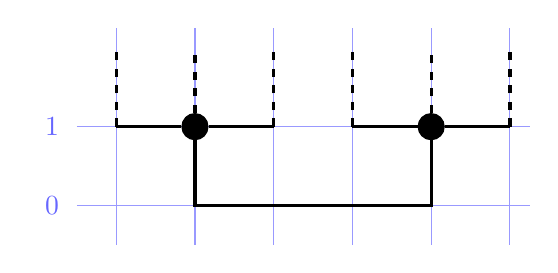
\begin{tikzpicture}[every node/.style={draw,circle,fill}]

\foreach \x in {-1,...,4}
	\draw[color=blue!40](\x,-1.5)--(\x,1.25);
\foreach \x in {-1,0}
	\draw[color=blue!40](-1.5,\x)--(4.25,\x);
\node[draw=none,fill=none,anchor=east,color=blue!60] at (-1.5,0) {1};
\node[draw=none,fill=none,anchor=east,color=blue!60] at (-1.5,-1) {0};
\node (v1) at (0,0) {};
\node (v2) at (3,0) {};
\draw[very thick] (v1) to(0,-1)-| (v2);
\coordinate (7) at (-1,0);
\coordinate (8) at (1,0) {};
\coordinate (9) at (2,0) {};
\coordinate (10) at (4,0) {};
\coordinate (1) at (-1,1) {};
\coordinate (2) at (0,1) {};
\coordinate (3) at (1,1) {};
\coordinate (4) at (2,1) {};
\coordinate (5)at (3,1) {};
\coordinate (6)at (4,1) {};
\foreach \x/\y in {1/7,1/8,2/9,2/10}
	\draw[very thick] (v\x) to (\y);
\foreach \x/\y in {7/1,v1/2,8/3,9/4,v2/5,10/6}
	\draw[dashed,very thick] (\x) to (\y);
\end{tikzpicture}
\end{minipage}
\begin{minipage}{0.55\textwidth}
	\begin{itemize}[itemsep=-1pt]
		\item $d(v)=\dleft(v)+\dright(v)$
		\item $1\leq \dleft(v)$
		\item $3\leq \dright(v)$
		\item Plazierung der ersten beiden Knoten (\textbf{links})
	\end{itemize}
\end{minipage}\\
\begin{minipage}{2cm}
\end{minipage}
\begin{minipage}{0.35\textwidth}
	\usetikzlibrary{positioning}

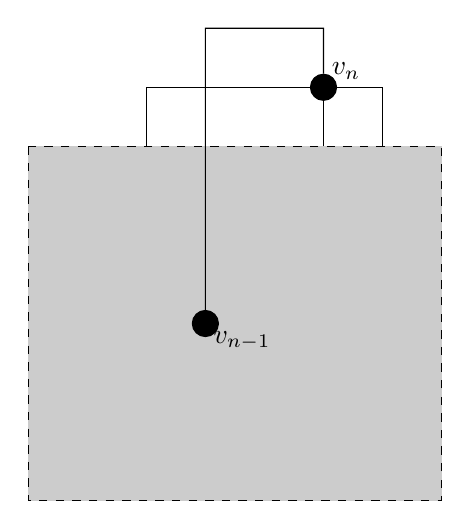
\begin{tikzpicture}[node distance=-0.2cm,scale=0.75]
\draw[fill=black!20,dashed] (-5,1) rectangle (2,-5);
\node[draw,fill,circle] (v1) at (-2,-2) {};
\node[draw,fill,circle] (v4) at (0,2) {};
\coordinate (v2) at (-2,3) {};
\draw  (v1) -- (v2)-|(v4);

\coordinate (v8) at (-3,1) {};
\coordinate (v6) at (1,1) {};
\coordinate (v5) at (0,1) {};
\draw  (v5) edge (v4);
\draw  (v6) |- (v4);
\draw  (v8) |- (v4);
\node[below right=of v1]{$v_{n-1}$};
\node[above right=of v4]{$v_{n}$};

\end{tikzpicture}
\end{minipage}
\begin{minipage}{0.6\textwidth}
	\begin{itemize}[itemsep=-1pt]
		\item für alle adjazenten Nachfolger werden jeweils die Gittervertikalen durch $v$ sowie, falls nötig, zwei neue links und rechts vom Layout reserviert
		\item alle anderen Knoten werden auf der Gitterhorizontalen mit $y(v_i)=i$ entsprechend der Anzahl der adjazenten Vorgänger plaziert
		\item $v_n$ kommt auf die Gitterhorizontale $y(t)=n$ (siehe links)
	\end{itemize}
\end{minipage}\\
\begin{itemize}
	\item die benötigte Gittergröße ist höchstens $(m-n+1)\times n$
		\begin{itemize}
			\item erste beiden Knoten brauchen Höhe $1$
			\item die weiteren Knoten erhöhen die Hähe um $1$
			\item der letzte Knoten erhöht die Höhe höchstens um $2$
			\item[$\Rightarrow$] Höhe $n$
			\item erste beiden Knoten brauchen Breite $\dright(v_1)+\dright(v_2)-2$
			\item die weiteren Knoten vergrößern die Breite um $\dright(v_i)-1$
			\item der letzte Knoten erhöht die Breite nicht
			\item[$\Rightarrow$] Breite$=\sum\limits_{v\in V}(\dright(v)-1)+1=m-n+1$
		\end{itemize}
\end{itemize}
\topbreak
\vspace*{-2\baselineskip}
\begin{itemize}[itemsep=-1pt]
	\item die Gesamtzahl der Knicke ist höchstens $2m-2n+4$ und keine Kante hat mehr als $2$ Knicke
		\begin{itemize}[itemsep=-1pt]
			\item für $v_1,v_2$ werden $\dright(v_1)+\dright(v_2)-1$ Knicke erzeugt
			\item für jeden Knoten $v\neq v_1,v_2,v_n$ werden $\dleft(v)-1+\dright(v) -1 =2d_G(v)-2$ Knicke erzeugt
			\item für $v_n$ werden $4$ Knicke benötigt, falls $d_G(v_n)=4$, sonst nur $d_G(v_n)-1$
			\item[$\Rightarrow$] maximal: $\sum\limits_{v\in V}d_G(v)-2)+4=2m-2n+4$
			\item erste und letzte Kante $\{v_1,v_2\}, \{v_{n-1},v_n\}$ haben maximal $2$ Knicke (Konstruktion)
			\item jede andere Kante hat höchstens einen Knick auf der Gitterhorizontalen durch beide Endknoten
		\end{itemize}
	\item ist $G$ planar und liegen $s,t$ auf der äußeren Facette\\
	$\Rightarrow$ für jede $st$-Ordnung $v_1,\dots,v_n$ liegt $v_i$ auf der äußeren Facette des von $v_1,\dots,v_{i-1}$ induzierten Teilgraphen, sowie die Vorgänger von $v_i$ bilden auf der äußeren Facette ein Intervall
	\item durch Einfügen von neuen Spalten direkt neben dem gerade zu platzierenden Knoten, berechnet der Algorithmus kreuzungsfreie, orthogonale Gitterlayouts
	\item gibt einen Graph, der $3$ Knicke an einer Kante braucht!
\end{itemize}
\subsection{Kombination der Komponentenlayouts (4. Schritt)}
\begin{minipage}{0.2\textwidth}
	\hspace*{1cm}\underline{Komponenten}\\
	\usetikzlibrary{positioning,calc}
\begin{tikzpicture}[every node/.style={draw,circle},scale=0.75]
\def\s{1.5}

\foreach \x/\y/\l in {0/0/2,0/1/3,1/2/4,1/3/5,1/4/1,2/1/a,3/0/b}
	\node (\l) at (\x*\s,\y*\s) {};
\foreach \a/\b in {1/5,5/4,4/3,3/2,4/a,a/b}
	\draw(\a)--(\b);
\draw[color=blue,dashed](1)to[out=200](2);
\draw[color=blue,dashed](5)to[out=225,in=45](2);
\draw[color=blue,dashed](5)to[out=200,in=90](3);
\draw[color=blue,dashed](4)to[out=0,in=90](b);
\end{tikzpicture}
\end{minipage}
\begin{minipage}{0.3\textwidth}
	\centering \underline{$st$-Ordnungen}\\
	\usetikzlibrary{positioning,calc}
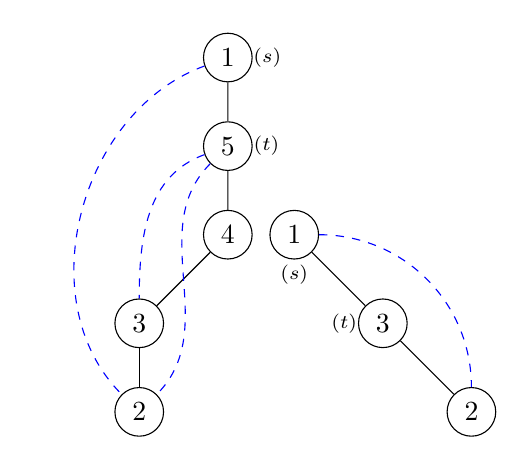
\begin{tikzpicture}[every node/.style={draw,circle},node distance=0cm,scale=0.75]
\def\s{1.5}

\foreach \x/\y/\l in {0/0/2,0/1/3,1/2/4,1/3/5,1/4/1}
	\node (\l) at (\x*\s,\y*\s) {$\l$};

\node[right=of 5,xshift=-0.2cm,draw=none] {\scriptsize$(t)$};
\node[right=of 1,xshift=-0.2cm,draw=none] {\scriptsize$(s)$};

\foreach \a/\b in {1/5,5/4,4/3,3/2}
	\draw(\a)--(\b);
\draw[color=blue,dashed](1)to[out=200](2);
\draw[color=blue,dashed](5)to[out=225,in=45](2);
\draw[color=blue,dashed](5)to[out=200,in=90](3);

\node (1) at (1.75*\s,2*\s) {$1$};
\node (3) at (2.75*\s,1*\s) {$3$};
\node (2) at (3.75*\s,0*\s) {$2$};

\foreach \a/\b in {1/3,3/2}
	\draw(\a)--(\b);
\draw[color=blue,dashed](1)to[out=0,in=90](2);

\node[left=of 3,xshift=0.2cm,draw=none] {\scriptsize$(t)$};
\node[below=of 1,yshift=0.2cm,draw=none] {\scriptsize$(s)$};
\end{tikzpicture}
\end{minipage}
\begin{minipage}{0.3\textwidth}
	\centering \underline{kombinierte Layouts}\\
	\usetikzlibrary{positioning,calc}
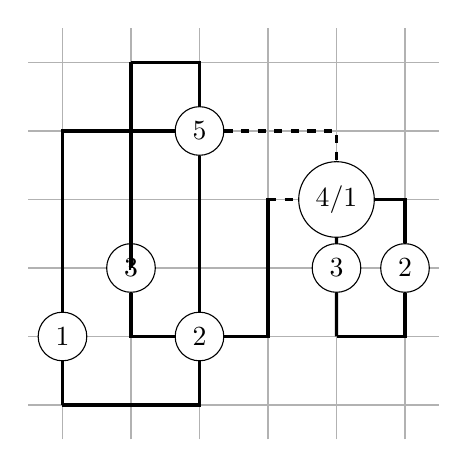
\begin{tikzpicture}[every node/.style={draw,circle},node distance=0cm,scale=0.58]
\def\s{1.5}
\draw[color=black!30,step=\s](-0.5*\s,-0.5*\s)grid(5.5*\s,5.5*\s);
\foreach \x/\y/\l in {2/1/2,1/2/3,2/4/5,0/1/1}
	\node[fill=white] (\l) at (\x*\s,\y*\s) {$\l$};

%\node[right=of 5,xshift=-0.2cm,draw=none] {\scriptsize$(t)$};
%\node[right=of 1,xshift=-0.2cm,draw=none] {\scriptsize$(s)$};

\foreach \a/\b in {5/1,2/3}
	\draw[very thick](\a)-|(\b);
%\draw[color=blue,dashed](1)to[out=200](2);
%\draw[color=blue,dashed](5)to[out=225,in=45](2);
%\draw[color=blue,dashed](5)to[out=200,in=90](3);
\draw[very thick](2)-|(3*\s,3*\s);
\draw[very thick](3)-|(1*\s,5*\s);
\draw[very thick](5)|-(1*\s,5*\s);
\draw[very thick](1)--(0*\s,0*\s);
\draw[very thick](2)|-(0*\s,0*\s);
\draw[very thick](2)--(5);

\node[fill=white] (3) at (4*\s,2*\s) {$3$};
\node[fill=white] (41) at (4*\s,3*\s) {$4/1$};
\node[fill=white] (2) at (5*\s,2*\s) {$2$};

\foreach \a/\b in {41/2}
	\draw[very thick](\a)-|(\b);
\draw[very thick](3)--(4*\s,1*\s);
\draw[very thick](2)|-(4*\s,1*\s);
\draw[very thick](3)--(41);

\draw[very thick,dashed](3*\s,3*\s)|-(41);
\draw[very thick,dashed](5)-|(41);

\end{tikzpicture}
\end{minipage}